\chapter{Eigenes Verfahren}\label{chp:EigVerfahren}
Diese Arbeit besteht aus drei gro�e Hauptschritte, n�mlich Hintergrundsubtraktion, Sch�tzung der K�rperhalterung mit Histogrammanalyse und Erkennung au�ergew�hnlicher Situation mit Fuzzylogik  

\section{Hintergrundsubtraktion}
In dieser Masterarbeit ist Hintergrundsubtraktion ein wichtiger Baustein. Ein gro�es Problem ist wie einer korrekte Hintergrund erstellt werden kann, damit man sich bewegtes Objekt robust erkennen kann. F�r diese Arbeit wurden verschiedenen moderne Methoden (Gaussian Mixture Model, Kern Density Estimation und Vibe) ausprobiert und verglichen. Die alle genannte Methoden wurden schon in ~\ref{sec:Grundlage1} theoretisch beschrieben. In diesem Abschnitt geht es um Bewertungen von Hintergrundsubtraktionsverfahren. Bei \acs{GMM} wird eine Mischung von 5-Gau�schen Verteilung modelliert und eine Anzahl von 100 letzte Frames wird als "History"\ angewendet. Mit dem Lernrate $0.01$ funktioniert das \acs{GMM} Verfahren gut in unserem Test. F�r das \acs{AGMM} nehmen wir auch die gleiche Parameters, um das Vergleichen der Hintergrundsubtraktionsverfahren objektiv zu bewerten. Bei \acs{KDE} handelt es sich um eine Berechnung von Intensit�tswerte f�r einen Pixel, deshalb wird nur ein Parameter von 100 als "History" wie bei \acs{AGMM} in diesem Fall eingesetzt. Wie in \cite{barnich2009vibe} schon gemeint, Vibe ist ein nicht-parametrisches Verfahren und weshalb kein Parameter wird hier gebraucht.

\begin{figure}[htpb]
	\centering
	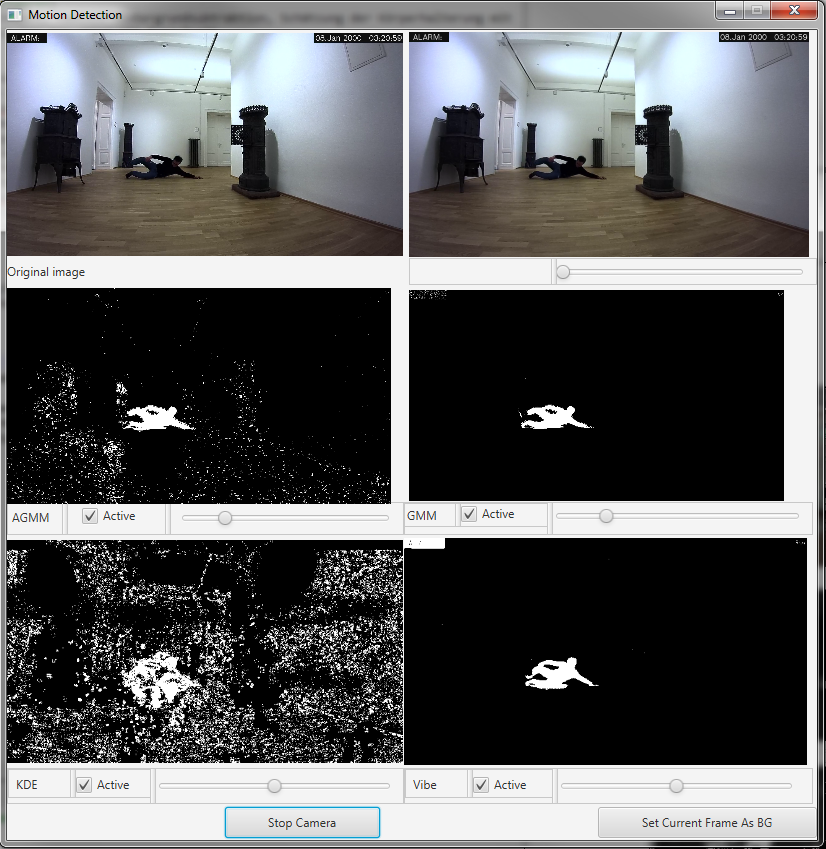
\includegraphics[width=1\textwidth]{fig/motiondetrection7.png}
	\caption{Vergleichen von verschiedene Techniken an Hintergrundsubtraktion} 
	\label{fig:compare_bgsubtraction}
\end{figure}




\subsection{Vergleichen verschiedener Methoden}
\subsection{Eigene Methode}
\subsection{Ergebnisse der eigene Hintergrundsubtraktion}
\section{Sch�tzung der K�rperhalterung mit Histogrammanalyse}
\section{Erkennung au�ergew�hnlicher Situation}